%\documentclass[12pt, preprint,numberedappendix]{emulateapj}
%\documentclass[12pt, preprint]{aastex}
%\documentclass[apj]{emulateapj}
\documentclass[12pt, letterpaper]{article}

%\newcommand\submitms{n}		% set to y to follow AAS ``ms'' names, etc.
%\newcommand\bibinc{n}		% set to y if bib pasted in .tex, set to n to use bibtex


%\usepackage{pdfsync}
%\usepackage{subeqnarray}
\usepackage[top=0.9in, bottom=0.6in, left=1in, right=1in]{geometry}
\usepackage{natbib}
\usepackage{color}
\usepackage{graphicx}
\usepackage{fancyhdr}
\usepackage[T1]{fontenc}
\usepackage{titling}
\usepackage{sectsty}
\usepackage{sidecap}
\usepackage{placeins}
\usepackage{indentfirst}
\usepackage{wrapfig}
\usepackage[font={footnotesize}]{caption}
\usepackage{multicol}
\setlength{\droptitle}{-7em}
\setlength{\abovecaptionskip}{-2.5ex}
\setlength{\belowcaptionskip}{-2.5ex}
%\pagenumbering{gobble}
\pagestyle{fancy}
\lhead{Ana-Maria Piso}
\rhead{Sagan Fellowship Previous and Current Research Statement}
\date{}
%\rhead{\thepage}


%\bibliographystyle{apj}

\title{\large PCEPS Research Statement: \\
Dynamics and Chemistry: The Disk-Planet Connection \vspace{-2.8ex}}
\author{\normalsize Ana-Maria Piso \vspace{-2.8ex}}

%\newenvironment{packed_item}{
%\begin{itemize}
%  \setlength{\itemsep}{1pt}
%  \setlength{\parskip}{0pt}
%  \setlength{\parsep}{0pt}
%}{\end{itemize}}

\begin{document}
\maketitle

%\slugcomment{Draft Modified \today}

\vspace{-1.5cm}

Within the last two decades, more than one thousand extrasolar planets have been discovered. Their diversity in terms of mass, radius, location and composition provides an exciting field of research, with the eventual goal of finding planets that are similar to our own Earth and may sustain life. For this purpose, it is thus crucial to explore and understand how planets obtain their compositions. Both terrestrial and giant planets are born in protoplanetary disks, which implies that their composition is determined by and tightly linked to the structure and composition of the disk. In my past, current and future research, I approach this intricate disk-planet link from three directions: (1) by exploring the core accretion mechanism, specifically calculating the minimum required core mass to form a gas giant before the dissipation of the gas in the protoplanetary disk, (2) by understanding how disk chemistry and dynamics affect the snowline locations of volatiles in disks, and (3) by investigating the role of disk volatile chemistry and dynamics in shaping the compositions of nascent planets.

\noindent \underline{\textbf{Previous Research}}

%Planets are born in protoplanetary disks, which means that their structure and composition are determined by and highly connected to the chemical composition and structure of the disk in which they form. In my current and previous research, I have approached this intricate disk-planet link from two directions: (1) by exploring the core accretion mechanism, specifically calculating the minimum required core mass to form a gas giant before the dissipation of the gas in the protoplanetary disk, and (2) by understanding how disk chemistry and dynamics shape the snowline locations of volatiles in disks, which has direct implications for the chemical composition of extrasolar planet (exoplanet) atmospheres.

\textbf{1. Minimum Core Masses for Giant Planet Formation.} Gas giants are widely believed to form through core accretion, a theory in which solid protoplanetary cores grow large enough to accumulate a massive atmosphere. Core accretion is particularly challenging in the outer parts of a disk, where long dynamical times make it difficult for a core to grow fast enough before the gas disk dissipates on a timescale of a few million years. At the same time, however, giant planets on wide orbits have been discovered in recent years, which poses the question of how these planets have formed. I addressed this issue by calculating the minimum (critical) core mass $M_{\rm crit}$ required to form a giant planet during the lifetime of the protoplanetary disk. This minimum applies when solid cores no longer accrete planetesimals, as this would heat the gaseous envelope and inhibit the atmosphere's ability to cool and contract. I thus considered envelopes accreting around fully formed cores at distances between 5 and 100 astronomical units (AU) from their host star. To obtain robust quantitative results for $M_{\rm crit}$, I assumed a realistic equation of state (EOS) for the nebular gas and realistic opacities that take into account grain growth. I found that $M_{\rm crit}$ decreases with semimajor axis, from 8 Earth masses ($M_{\oplus}$) at 5 AU to 5 $M_{\oplus}$ at 100 AU. These results are lower than the typically quoted value of 10 $M_{\oplus}$, and may be up to one order of magnitude lower if grain coagulation is taken into account. Thus our studies clearly challenge previous claims that core accretion cannot operate in the outer parts of protoplanetary disks, reopening the case for in situ formation of wide-separation gas giants. 

In the second part of my talk, I will transition to protoplanetary disks, and to how their composition and evolution may affect the formation and chemical composition of giant planets. As the C/O ratio is an important signature of giant planet atmospheres, I will discuss how the snowline locations of the main C and O carriers, i.e. H2O, CO2 and CO, are affected by radial drift of solids and viscous gas accretion. Compared to a static disk, these two effects move the snowlines inwards by ~50%. This affects the C/O ratio in gas and dust throughout the disk, and thus has direct implications in shaping the composition of nascent giant planets.
\underline{\textbf{B. Nitrogen Abundance and Ice Binding Energies}}

Aside from the main C and O carriers, nitrogen (N) bearing species are important to study. Nitrogen is highly abundant in the Solar system $[18]$ and disks, and primarily found as N$_2$. Because of the high volatility of N$_2$, the gas phase nitrogen-to-oxygen (N/O) ratio in the outer disk may be even more enhanced than the C/O ratio. Giant planets that form at wide separations should thus have an excess of N in their atmospheres, which could be used to trace their formation origin. In $[19]$, we quantify this effect in disks. We find that the N/O ratio in gas is significantly larger than the Solar abundance, and indeed exceeds the C/O ratio in the outer disk. We can thus set the stage to answer one of our main questions, i.e. back-track the planet formation location based on planet composition. In this study we also explore the effects of assuming that N$_2$ is bound to water ice instead of pure N$_2$, and the presence of some N in the form of NH$_3$. In either case, the general result of a large N/O enhancement in the outer disk is preserved. \\
\underline{\textbf{C. Self-consistent C/N/O Calculation}}

As shown in Figure 2, our current drift-desorption model can only provide us with upper estimates for C/O (or N/O) ratios. We plan to enhance this model by performing the time-dependent calculation that accounts for the relative motion of the desorbed ices and the overall nebular gas, the time evolution of the dust surface density,  and radial gas diffusion; all these effects will change the volatile abundances and the C/O ratio in time. We have developed a code that evolves the dust surface density for a particle of fixed size. Next, we will treat  each species in gaseous and solid forms as two fluids that are interchanging. Following $[20]$, we will use advection-like equations to solve for their separate time-dependent abundance. 

\noindent \underline{\textbf{Proposed Research}}

%Within the last two decades, more than one thousand extrasolar planets have been discovered. Their diversity in terms of mass, radius, location and composition provides an exciting field of research, with the eventual goal of finding planets that are similar to our own Earth and may sustain life. For this purpose, it is thus crucial to explore and understand how planets obtain their compositions. Both terrestrial and giant planets are born in protoplanetary disks, which implies that their composition is determined by and tightly linked to the structure and composition of the disk. 
As shown in my work on the minimum core mass of gas giants and snowlines in disks, planet formation depends sensitively on disk physics and chemistry. I propose to develop a holistic chemo-dynamical framework to explore how disk dynamics and chemistry, as well as the dynamics of nascent planets and planetesimals, regulate the compositions of mature giant planets. Such a model will enhance our understanding of planetary structures by enabling us to predict what kind of planet compositions result from planet formation in different parts of the disk. Furthermore, this work provides essential context for characterizing the planets that instruments such as the James Webb Space Telescope (JWST) and the Transiting Exoplanet Survey Satellite (TESS) will one day discover. 

\textbf{1. Coupled Chemical and Dynamical Disk Evolution.} Chemical and dynamical processes in a protoplanetary disk affect the disk structure and composition, and thus the composition of nascent planets. Chemical abundances vary significantly across a typical disk, due to steep gradients in temperature, density and radiation. The complexity of disk chemistry means that coupling it with dynamical processes is non-trivial. Through analytical and numerical calculations, I will first explore a range of dynamical processes that may affect the distribution of volatiles in disks, expanding and generalizing the framework I developed during my dissertation research. I will couple this dynamical model with a simple chemical network, then use more complex chemical networks to develop a simplified time-dependent chemistry, informed by results from state-of-the-art disk chemistry models (that can only be run on static disks). This will show how the snowline locations of volatiles, as well as the chemical composition of the disk gas and dust evolve, which has direct implications on the compositions of young planets.

\textbf{2. Planet and Planetesimal Migration.} Giant planets can migrate through the disk while still accumulating gas, which will change their atmospheric composition since the disk chemical abundances are different at different disk locations. Additionally, giant planets may still accumulate planetesimals while accreting nebular gas. The final composition of a planet?s atmosphere will thus depend on how much gas and solids are accreted in this stage. I will add planet dynamical effects such as migration and planetesimal accretion in the chemical and dynamical model developed in part 1, and quantify how these processes affect the chemical composition of gas giant envelopes. 

\textbf{3. Model Planet Populations.} The results from parts 1 and 2 will feed into a large planet synthesis model, in which I will use a grid of different initial disk and planetary embryo conditions. For this computationally expensive step, I will only include the processes that I have identified to be the most important in the local simulations from steps 1 and 2. This will allow me to constrain a planet?s formation location based on its chemical composition. Comparing my results with future JWST observations of atmospheric spectra will lead to great scientific strides in understanding the complex connection between protoplanetary disks and the formation, evolution and composition of exoplanets.

%\begin{figure}[h!]
%\centering
%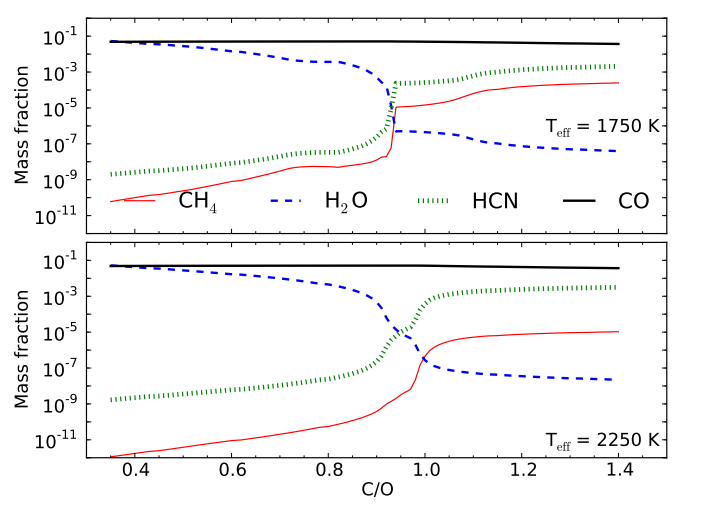
\includegraphics[width=0.7\textwidth]{CO_abundances}
%%\vspace{-0.5in}
%\caption{TBD}
%\label{fig:CO}
%\end{figure}


%\if\bibinc n
%\bibliography{refs}
%\fi
%\FloatBarrier
%\def\bibfont{\footnotesize}
%\setlength{\bibsep}{0.0pt}

\footnotesize

%\textbf{References} \\
%\begin{thebibliography} {9}
%\begin{multicols}{2}
%\noindent 
%$[1]$ Pollack, et al. 1996, Icarus, 124, 62 \\
%$[2]$ Marois, C.,  et al.. 2008, Science, 322, 1348 \\
%$[3]$ \textbf{Piso, A.-M. A.},\&Youdin,A.N. 2014,ApJ,786,21 \\
%$[4]$ \textbf{Piso, A.-M. A.}, et al. 2015, ApJ, 800, 82 \\
%$[5]$ Bodenheimer, P.\&Pollack, J. 1986, Icarus, 67, 391 \\
%$[6]$ Rafikov, R. R. 2006, ApJ, 648, 666 \\
%$[7]$ Bell, K. R. \& Lin, D. N. C. 1994, ApJ, 427, 987 \\
%$[8]$ Lee, E. J., et al. 2014, ApJ, 797, 95 \\ 
%$[9]$ Lee, E. J., \& Chiang, E. 2015, ApJ, 811, 41 \\
%$[10]$ Saumon, et al. 1995, ApJS, 99, 713 \\
%$[11]$ D'Alessio, P., et al. 2001, ApJ, 553, 321 \\
%$[12]$ Henning,T.,\&Semenov, D. 2013, ChRv, 113, 9016 \\
%$[13]$ Qi, C., et al. 2013, Science, 341, 630 \\
%$[14]$ Zhang, K., et al. 2013, ApJ, 766, 82 \\
%$[15]$ Molli{\`e}re, P., et al. 2015, ApJ, 813, 1 \\
%$[16]$ \"Oberg, K. I., et al. 2011, ApJ, 743, L16 \\
%$[17]$ \textbf{Piso, A.-M. A.}, et al. ApJ (under review) \\
%$[18]$ Lodders, K. 2009, arXiv:0910.0811 \\
%$[19]$ \textbf{Piso, A.-M. A.}, et al. (in prep) \\
%$[20]$ Ciesla, F. J. \& Cuzzi, J. N. 2006, Icarus, 181, 178
%
%
%%Stevenson, D. J. 1982, Planet. Space Sci., 30, 755 \\
%
%\end{multicols}
%\end{thebibliography}

%\bibliographystyle{abbrv}
%\bibliography{refs}


%\if\bibinc y
%\begin{thebibliography}
%\end{thebibliography}
%\fi


\end{document}